%%%%%%%%%%%%%%%%%%%%%%%%%%%%%%%%%%%%%%%%%
% Masters/Doctoral Thesis
% LaTeX Template
% Version 2.5 (27/8/17)
%
% This template was downloaded from:
% http://www.LaTeXTemplates.com
%
% Version 2.x major modifications by:
% Vel (vel@latextemplates.com)
%
% This template is based on a template by:
% Steve Gunn (http://users.ecs.soton.ac.uk/srg/softwaretools/document/templates/)
% Sunil Patel (http://www.sunilpatel.co.uk/thesis-template/)
%
% Template license:
% CC BY-NC-SA 3.0 (http://creativecommons.org/licenses/by-nc-sa/3.0/)
%
%%%%%%%%%%%%%%%%%%%%%%%%%%%%%%%%%%%%%%%%%

%----------------------------------------------------------------------------------------
%	PACKAGES AND OTHER DOCUMENT CONFIGURATIONS
%----------------------------------------------------------------------------------------

\documentclass[
11pt, % The default document font size, options: 10pt, 11pt, 12pt
oneside, % Two side (alternating margins) for binding by default, uncomment to switch to one side
english, % ngerman for German
%singlespacing, % Single line spacing, alternatives: onehalfspacing or doublespacing
%draft, % Uncomment to enable draft mode (no pictures, no links, overfull hboxes indicated)
%nolistspacing, % If the document is onehalfspacing or doublespacing, uncomment this to set spacing in lists to single
%liststotoc, % Uncomment to add the list of figures/tables/etc to the table of contents
%toctotoc, % Uncomment to add the main table of contents to the table of contents
%parskip, % Uncomment to add space between paragraphs
%nohyperref, % Uncomment to not load the hyperref package
headsepline, % Uncomment to get a line under the headeroooo
%chapterinoneline, % Uncomment to place the chapter title next to the number on one line
%consistentlayout, % Uncomment to change the layout of the declaration, abstract and acknowledgements pages to match the default layout
]{MastersDoctoralThesis} % The class file specifying the document structure

\usepackage[utf8]{inputenc} % Required for inputting international characters
\usepackage[T1]{fontenc} % Output font encoding for international characters

\usepackage{mathpazo} % Use the Palatino font by default

\usepackage[backend=bibtex,style=authoryear,natbib=true]{biblatex} % Use the bibtex backend with the authoryear citation style (which resembles APA)

\addbibresource{Project.bib} % The filename of the bibliography

\usepackage[autostyle=true]{csquotes} % Required to generate language-dependent quotes in the bibliography

\usepackage{titlesec}
\titleformat{\chapter}{}{}{0em}{\bf\LARGE}

\usepackage[export]{adjustbox}[2011/08/13]



%----------------------------------------------------------------------------------------
%	MARGIN SETTINGS
%----------------------------------------------------------------------------------------

\geometry{
	paper=a4paper, % Change to letterpaper for US letter
	inner=2.5cm, % Inner margin
	outer=3.8cm, % Outer margin
	bindingoffset=.5cm, % Binding offset
	top=1.5cm, % Top margin
	bottom=1.5cm, % Bottom margin
	%showframe, % Uncomment to show how the type block is set on the page
}

%----------------------------------------------------------------------------------------
%	THESIS INFORMATION
%----------------------------------------------------------------------------------------

\thesistitle{Using acoustic monitoring and machine learning to automate the detection of illegal activity in Costa Rica} % Your thesis title, this is used in the title and abstract, print it elsewhere with \ttitle
\supervisor{Dr. Cristina \textsc{Banks-Leite}\break
Dr. James \textsc{Rosindell}} % Your supervisor's name, this is used in the title page, print it elsewhere with \supname
\examiner{} % Your examiner's name, this is not currently used anywhere in the template, print it elsewhere with \examname
\degree{Master of Science} % Your degree name, this is used in the title page and abstract, print it elsewhere with \degreename
\author{Jacob \textsc{Griffiths}} % Your name, this is used in the title page and abstract, print it elsewhere with \authorname
\addresses{} % Your address, this is not currently used anywhere in the template, print it elsewhere with \addressname

\subject{Computational Biology} % Your subject area, this is not currently used anywhere in the template, print it elsewhere with \subjectname
\keywords{} % Keywords for your thesis, this is not currently used anywhere in the template, print it elsewhere with \keywordnames
\university{\href{https://www.imperial.ac.uk}{Imperial College London}} % Your university's name and URL, this is used in the title page and abstract, print it elsewhere with \univname
\department{\href{https://www.imperial.ac.uk/life-sciences/}{Department of Life Sciences}} % Your department's name and URL, this is used in the title page and abstract, print it elsewhere with \deptname
\group{\href{https://www.imperial.ac.uk/study/pg/life-sciences/computational-methods-ecology-evolution/}{Computational Methods in Ecology and Evolution}} % Your research group's name and URL, this is used in the title page, print it elsewhere with \groupname
\faculty{\href{https://www.imperial.ac.uk/natural-sciences/}{Faculty of Natural Sciences}} % Your faculty's name and URL, this is used in the title page and abstract, print it elsewhere with \facname

\AtBeginDocument{
\hypersetup{pdftitle=\ttitle} % Set the PDF's title to your title
\hypersetup{pdfauthor=\authorname} % Set the PDF's author to your name
\hypersetup{pdfkeywords=\keywordnames} % Set the PDF's keywords to your keywords
}

\linespread{1.25}


\begin{document}


\frontmatter % Use roman page numbering style (i, ii, iii, iv...) for the pre-content pages

\pagestyle{plain} % Default to the plain heading style until the thesis style is called for the body content

%----------------------------------------------------------------------------------------
%	TITLE PAGE
%----------------------------------------------------------------------------------------

\begin{titlepage}
\begin{center}

\vspace*{.06\textheight}
{\scshape\LARGE \univname\par}\vspace{1.5cm} % University name
\textsc{\Large Thesis}\\[0.5cm] % Thesis type

\HRule \\[0.4cm] % Horizontal line
{\huge \bfseries \ttitle\par}\vspace{0.4cm} % Thesis title
\HRule \\[1.5cm] % Horizontal line

\begin{minipage}[t]{0.4\textwidth}
\begin{flushleft} \large
\emph{Author:}\\
\href{https://www.linkedin.com/in/jacob-griffiths-7b7438b4/}{\authorname} % Author name - remove the \href bracket to remove the link
\end{flushleft}
\end{minipage}
\begin{minipage}[t]{0.4\textwidth}
\begin{flushright} \large
\emph{Supervisors:} \\
\href{https://www.imperial.ac.uk/people/c.banks}{\supname} % Supervisor name - remove the \href bracket to remove the link
\end{flushright}
\end{minipage}\\[3cm]

\vfill

\large \textit{A thesis submitted in partial fulfilment of the requirements \\ for the degree of Master of Science at Imperial College London}\\[0.3cm] % University requirement text
\textit{Formatted in the journal style of}\\[0.3cm]
\textit{Submitted for the MSc in Computational Methods in Ecology and Evolution}\\[0.3cm]

\deptname\\[2cm] % Research group name and department name

\vfill

{\large \today}\\[4cm] % Date
%\includegraphics{Logo} % University/department logo - uncomment to place it

\vfill
\end{center}
\end{titlepage}

%----------------------------------------------------------------------------------------
%	DECLARATION PAGE
%----------------------------------------------------------------------------------------

\begin{declaration}
\addchaptertocentry{\authorshipname} % Add the declaration to the table of contents
\noindent I, \authorname, declare that this thesis titled, \enquote{\ttitle} and the work presented in it are my own. I confirm that:

\begin{itemize}
\item This work was done wholly or mainly while in candidature for a research degree at this University.
\item Where any part of this thesis has previously been submitted for a degree or any other qualification at this University or any other institution, this has been clearly stated.
\item Where I have consulted the published work of others, this is always clearly attributed.
\item Where I have quoted from the work of others, the source is always given. With the exception of such quotations, this thesis is entirely my own work.
\item I have acknowledged all main sources of help.
\item Where the thesis is based on work done by myself jointly with others, I have made clear exactly what was done by others and what I have contributed myself.\\
\end{itemize}

\noindent Signed:\\
\rule[0.5em]{25em}{0.5pt} % This prints a line for the signature

\noindent Date:\\
\rule[0.5em]{25em}{0.5pt} % This prints a line to write the date
\end{declaration}

\cleardoublepage

%----------------------------------------------------------------------------------------
%	QUOTATION PAGE
%----------------------------------------------------------------------------------------

%\vspace*{0.2\textheight}

%\noindent\enquote{\itshape Thanks to my solid academic training, today I can write hundreds of words on virtually any topic without possessing a shred of information, which is how I got a good job in journalism.}\bigbreak

%\hfill Dave Barry

%----------------------------------------------------------------------------------------
%	ABSTRACT PAGE
%----------------------------------------------------------------------------------------

\begin{abstract}
\addchaptertocentry{\abstractname} % Add the abstract to the table of contents
Abstract written here
\end{abstract}

%----------------------------------------------------------------------------------------
%	ACKNOWLEDGEMENTS
%----------------------------------------------------------------------------------------

\begin{acknowledgements}
\addchaptertocentry{\acknowledgementname} % Add the acknowledgements to the table of contents
Write acknowledgements here
\end{acknowledgements}

%----------------------------------------------------------------------------------------
%	LIST OF CONTENTS/FIGURES/TABLES PAGES
%----------------------------------------------------------------------------------------

\tableofcontents % Prints the main table of contents

\listoffigures % Prints the list of figures

\listoftables % Prints the list of tables

%----------------------------------------------------------------------------------------
%	ABBREVIATIONS
%----------------------------------------------------------------------------------------

\begin{abbreviations}{ll} % Include a list of abbreviations (a table of two columns)

\textbf{PAM} & \textbf{P}assive \textbf{A}udio \textbf{M}onitoring\\
\textbf{MFC} & \textbf{M}el \textbf{F}requency \textbf{C}epstrum\\
\textbf{MFCCs} & \textbf{M}el \textbf{F}requency \textbf{C}epstrum \textbf{C}oefficients\\
\textbf{CNN} & \textbf{C}onvolutional \textbf{N}eural \textbf{N}etwork\\

\end{abbreviations}

%----------------------------------------------------------------------------------------
%	PHYSICAL CONSTANTS/OTHER DEFINITIONS
%----------------------------------------------------------------------------------------

%\begin{constants}{lr@{${}={}$}l} % The list of physical constants is a three column table

 %The \SI{}{} command is provided by the siunitx package, see its documentation for instructions on how to use it

%Speed of Light & $c_{0}$ & \SI{2.99792458e8}{\meter\per\second} (exact)\\
%Constant Name & $Symbol$ & $Constant Value$ with units\\

%5\end{constants}

%----------------------------------------------------------------------------------------
%	SYMBOLS
%----------------------------------------------------------------------------------------

%\begin{symbols}{lll} % Include a list of Symbols (a three column table)

%$a$ & distance & \si{\meter} \\
%$P$ & power & \si{\watt} (\si{\joule\per\second}) \\
%Symbol & Name & Unit \\

%\addlinespace % Gap to separate the Roman symbols from the Greek

%$\omega$ & angular frequency & \si{\radian} \\

%\end{symbols}

%----------------------------------------------------------------------------------------
%	DEDICATION
%----------------------------------------------------------------------------------------

%\dedicatory{For/Dedicated to/To my\ldots}

%----------------------------------------------------------------------------------------
%	THESIS CONTENT - CHAPTERS
%----------------------------------------------------------------------------------------

\mainmatter % Begin numeric (1,2,3...) page numbering

\pagestyle{thesis} % Return the page headers back to the "thesis" style

% Include the chapters of the thesis as separate files from the Chapters folder
% Uncomment the lines as you write the chapters

% Chapter Template

\chapter{Introduction} % Main chapter title

\label{Introduction}


\section{Biodiversity loss}

It is well documented that global biodiversity loss is accelerating. Anthropogenic factors are often touted as the leading cause, either directly through deforestation and hunting, or indirectly through climate change and the introduction of invasive species \citep{Chiarucci2011, Doherty2016, Newbold2015}. A meta-analysis by \cite{DeVos2015} gave an arguably conservative estimate of current biodiversity loss as being 1,000 times greater than the background 'natural' rate, with a magnitude of 10,000 times greater also being plausible \citep{Ceballos2015}. This alarming rate of loss not only affects the lost taxa themselves, but can also lead to extensive reduction in ecosystem multifunctionality, typically impacting poorer human communities \citep{Chiarucci2011, Allan2015, Fanin2018, Cardinale2012, Fanin2018}.\\

\noindent Tropical forests are no exception to this global trend. In addition to the adverse effects of deforestation on biodiversity, it is thought that other forms of anthropogenic disturbance, such as vehicles, hunting, and light pollution, can double the biodiversity loss \citep{Barlow2016}.

\section{Difficulties of measuring biodiversity and its loss}

Whilst it is universally agreed that biodiversity is being lost \citep{Cardinale2012, Ceballos2015, Fanin2018}, measuring this can be inconsistent and even erroneous \citep{Rocchini2018} for the following reasons. Firstly, only about 15\% of all species have been described, and therefore for the vast majority of species on Earth, there is no census data \citep{Chapman2009}. Secondly, of those that have been described, very little is known of their distribution, population size, ecology, and life histories, with many species only known by a single specimen \citep{Chapman2009}. Finally, of those species that have been described and studied in greater depth, there are inconsistencies in survey methods and often a lack of baseline measures to compare to \citep{TheRoy2003}.  The survey method deemed 'best' is often specific to a certain level of organisation and spatial scale of interest, such as satellite imagery and ground surveys for rainforest plant surveys. Despite the challenges and shortcomings associated with measuring biodiversity loss, it is indisputable that its acceleration is rapid, making urgent the development of programmes to assess and monitor biodiversity which are suitable for the answering of large-scale ecological questions \citep{Chiarucci2011, }.
Whilst it is universally agreed that biodiversity is being lost \citep{Cardinale2012, Ceballos2015, Fanin2018}, measuring this can be inconsistent and even erroneous \citep{Rocchini2018} for the following reasons. Firstly, only about 15\% of all species have been described, and therefore for the vast majority of species on Earth, there is no census data \citep{Chapman2009}. Secondly, of those that have been described, very little is known of their distribution, population size, ecology, and life histories, with many species only known by a single specimen \citep{Chapman2009}. Finally, of those species that have been described and studied in greater depth, there are inconsistencies in survey methods and often a lack of baseline measures to compare to \citep{TheRoy2003, Rocchini2018}.  The survey method deemed 'best' is often specific to a certain level of organisation and spatial scale of interest, such as satellite imagery and ground surveys for rainforest plant surveys \citep{Rocchini2018}. Despite the challenges and shortcomings associated with measuring biodiversity loss, it is indisputable that its acceleration is rapid, making urgent the development of programmes to assess and monitor biodiversity which are suitable for the answering of large-scale ecological questions \citep{Chiarucci2011, Rocchini2018}.


\section{Costa Rica and conservation}

Costa Rica is no exception to the aforementioned trend of biodiversity loss \citep{Hobinger2012}, with the Osa Peninsula being an area of focus for recent studies as it contains a mixture of protected, partially-protected, and unprotected land, including three national parks, Corcovado, Piedras Blancas and the Terreba-Sierpe wetlands  \citep{Lawson2019}. Whilst protected areas have benefited some species, others, such as the Geoffroy’s spider monkey, \textit{Ateles geoffroyi}, are struggling. This is due to their diet, need for mature trees, and need for large areas to roam, with typical home ranges of 4 km$^2$, which is increasingly limiting their range and may be isolating populations, in turn reducing their survival and genetic variability \citep{Chapman1989}. \textit{A. geoffroyi} is classified as endangered by the International Union for Conservation of Nature (IUCN) due to a 50\% reduction in numbers over the last 45 years \citep{Cuaron2008}. This reduction may be negatively impacting other species, as \textit{A. geoffroyi} is known to disperse the seeds of up to 150 tree species \citep{VanRoosmalen1985, Pacheco2000}. As well as habitat fragmentation, \textit{A. geoffroyi} is being subjected to hunting in both protected and non-protected areas. \cite{Aquino2013} found hunted populations of \textit{A. geoffroyi} in Peru were 70-80\% less dense than non-hunted populations. Admittedly, the monitoring and prevention of hunting in protected areas is often difficult in large reserves, due to the limited resources available to both rangers and conservationists. However, a recent study by \cite{Hill2018} demonstrated that gunshots can be detected with acoustic sensors up to 1km away from the source, opening up the possibility of a more effective and cheaper migration strategy.

\section{Passive acoustic monitoring and its advantages}

Passive acoustic monitoring (PAM) is becoming an increasingly popular method for large-scale biodiversity monitoring, primarily due to its relatively low cost \citep{Browning2017, Gibb2019}. This involves deploying sound recorders in an environment and having them record for days or weeks at a time to either track a vocal species directly or to use a vocal species as a proxy for another species or the ecosystem as a whole. Previously, methods such as PAM have been greatly limited by high implementation costs, a lack of digitisation, and low data storage capacity \citep{Merchant2015}. However, advances over the last 10-15 years have reduced the impact of these constraints dramatically \citep{Hill2018, Gibb2019}. One audio sensor in particular that has been developed recently in a collaborative project between the University of Oxford and University of Southampton, AudioMoth, is making PAM not only a viable option for monitoring biodiversity loss, but also one of the best methods available \citep{Hill2018}. \\

\noindent In addition to the direct monitoring of biodiversity, PAM can also be used to track other acoustics which may be relevant to conservation, such as gunshots, which are generally associated with illegal hunting, particularly in protected areas. \cite{Astaras2017} used PAM in a national park in Cameroon to successfully monitor the rates of hunting in the area. They found that most hunting (68.6\%) occurred at night when ranger patrols were minimal, and that there was more illegal activity during the week. \cite{Astaras2017} therefore argue that the hunting is for the illegal meat trade rather than for sustenance or sport, as the meat is gathered during the week for the Saturday market days. The cost of the PAM equipment was recorded by \cite{Astaras2017} as being quite high, which may limit the availability of its implementation in other national parks. However, the recent development of much cheaper audio sensors by \cite{Hill2018} may aid the spread of these techniques in conservation areas around the world. Digitisation has also made PAM a more viable survey mehod as it allows significantly longer recording times and records the data in a more appropriate format for computer analysis \citep{Hill2018, Gibb2019}.


\section{Machine learning}

Once audio data are collected, ecological information can be extracted manually or automatically. Manual extraction involves either auditory or visual inspection of the data and classification of the sounds, which naturally incurs some bias based on the skill of the person performing the analysis \citep{Heinicke2015}. This may be a viable option with a skilled ecologist and a small dataset. However, the latter is becoming increasingly rare with advancing technology, and therefore the need for automated techniques is growing rapidly. Fortunately, automated techniques are experiencing notable improvement in terms of both accuracy and efficiency, largely due to the use of machine learning \citep{Digby2013}. Most automated tools utilise supervised machine learning and related methods, including artificial neural networks \citep{Walters2012}, random forest \citep{ZamoraGutierrez2016}, Hidden Markov Models \citep{Zilli2014}, and support vector machines \citep{Heinicke2015}. These methods commonly use libraries of species calls or other sounds to facilitate detection when presented with new recordings. Currently, the low accuracy of these systems means that full automation is rare, and manual validation is often required \citep{Kalan2016}. However, new methods such as unsupervised feature extraction \citep{Stowell2014} and deep convolutional neural networks \citep{Goeau2016} can learn to classify directly from spectrogram data, often making them more robust and resistant to noise. At present, the main limitation for deep convolutional neural networks is large, clean datasets to train on.



\section{Aims}

\begin{enumerate}
  \item To use data provided by \cite{Hill2018} to train a deep convolutional neural network that can detect gunshots in acoustic data
  \item To investigate the effectiveness of using machine learning in cases such as this
  \item To identify the presence of any spatio-temporal patterns of hunting on the Osa Peninsula
\end{enumerate}

% Chapter Template

\chapter{Methods} % Main chapter title

\label{Methods} % Change X to a consecutive number; for referencing this chapter elsewhere, use \ref{ChapterX}

%----------------------------------------------------------------------------------------
%	SECTION 1
%----------------------------------------------------------------------------------------

Sound is the propagation of waves of pressure through a medium. When a gun is fired, the vibrations produced alternately compress and rarefy the medium, leading to waves of high and low pressure that propagate in all directions \citep{Bradbury2011}. Over time and distance, these waves attenuate, their amplitude reducing as energy dissipates into the environment \citep{Russ2013}. The sound waves can then be transduced into an electrical signal.  To record digitally, the analogue signal is sampled at a certain rate (typically measured in thousands of samples per second, kHz) and bit-depth (number of possible amplitude levels, typically 16-bit), with both parameters being important for determining frequency and amplitude resolution respectively. The signal information is then electronically recorded in the time-amplitude domain and can be processed mathematically using a fast Fourier transform (FFT) to convert the amplitude data into frequency data \citep{Fourier1822, Cooley1964}. For a given time window in the recording, the FFT calculates the frequency components of the signal and their relative amplitudes, producing a frequency spectrum. For a visual representation of the whole recording, an FFT is calculated with an overlapping short sliding window across the length of the recording, producing a spectrogram \citep{TheRoy2003} This entire process is outlined in Figure ~\ref{fig:audio_analysis}.\\

\begin{figure}
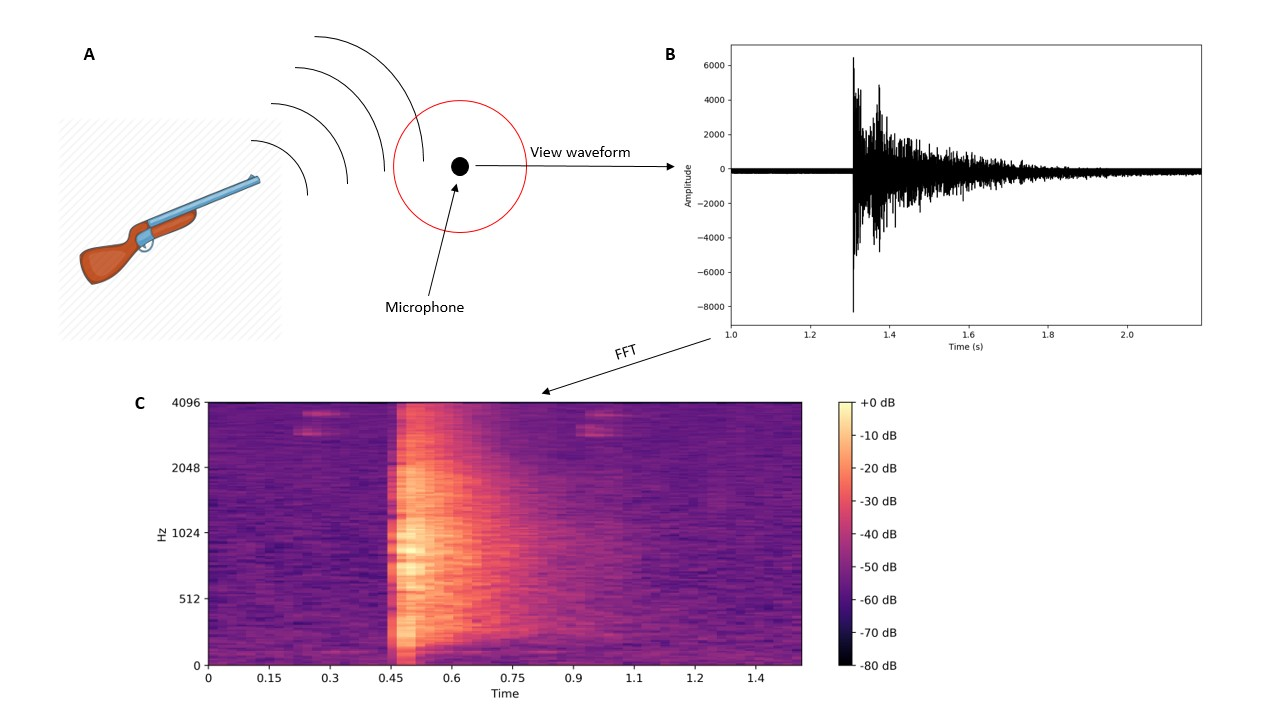
\includegraphics[width=1.2\textwidth,center]{Figures/audio_analysis}\caption[Analysis of acoustic data]{Recording and analysis of an acoustic signal. The emitted sound is transduced into an electrical signal by a microphone (\textbf{A}). In digital recording, the sound can be reconstructed in the time-amplitude domain (\textbf{B}) using the specified sampling rate (kHz). A frequency spectrum can then be produced using a fast Fourier transform (FFT), which calculates the signal’s frequency components and their relative amplitudes. Calculating FFT within a sliding window across the recording produces a spectrogram, with time on the x-axis, frequency on the y-axis, and with amplitude (energy) shown as colour intensity (\textbf{C})}\label{fig:audio_analysis}
\end{figure}

\noindent It is common in audio classification to plot a variant of the traditional spectrogram: the mel-frequency spectrogram. This involves calculating the mel-frequency cepstrum (MFC) which is a representation of the sound's power spectrum after the frequency has passed through a mathematical function. Mel-frequency cepstral coefficients (MFCCs) are the constituent coefficients of an MFC \citep{Xu2004}. They are calculated from a cepstral representation of the sound, with frequency bands equally spaced on the mel scale \citep{Stevens1937}. Spectrograms are fundamental to the analysis of acoustic data as they allow very specific sounds, such as a spider monkey call or a gunshot, to be visually identified and labelled, either manually or automatically.

\section{Data collection and preprocessing}


\subsection{Study site}

The audio data used in this study was collected at a study site in the Osa Peninsula, Costa Rica (Figure ~\ref{fig:peninsula_map}). This 2,500 km$^2$ site sits in a particularly diverse region, containing approximately 2.5\% of the world's species on less than 0.001\% of its land area \citep{Lawson2019}. Three national parks - Corcovado, Piedras Blancas, and the Terreba-Sierpe wetlands - and one forest reserve are represented within this study site. There has been significant landscape alterations in these areas which are inevitably brought about by an expanding human population and the introduction of agriculture and urbanisation \citep{Hobinger2012}.

\begin{figure}
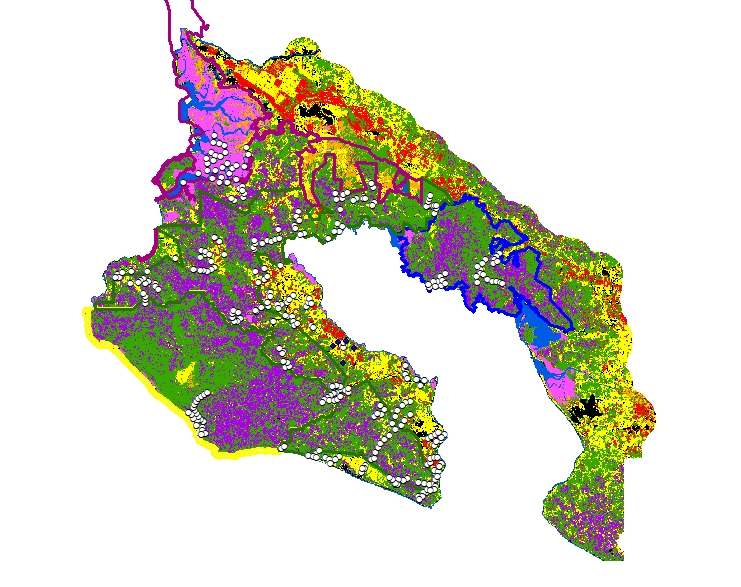
\includegraphics[width=1.2\textwidth,center]{Figures/peninsula_map}\caption[Map of Osa Peninsula]{Map of the study site in the Osa Peninsula \cite{Lawson2019} (NEED KEY/AREAS MARKED)}\label{fig:peninsula_map}
\end{figure}

\subsection{Sampling}

In this study, data from six AudioMoth acoustic sensors were collocted over six consecutive days, totalling 960 hours. These sensors covered protected forest reserve, protected grassland, and unprotected forest (TABLE), and were placed in areas known to be hotspots for hunting (personal communication, Jenna Lawson). Each device was set to record for three periods a day, 0500-0930, 1400-1830, and 2100-0300. These periods were chosen to coincide with the peak activity levels of \textit{A. geoffroyi} and their associated poaching. Sound was recorded continuously during these periods at a sample rate of 48 kHz and the devices were contained in waterproof casing to avoid damage. Every minute of audio data was saved in a separate file with the filename being a Unix hexadecimal timestamp. Where possible, trails and other areas of high human density were avoided.


\subsection{Training data}

\cite{Hill2018} provided the labelled audio data which was used in their study and was used in this study to train the neural network. The data was collected using 36 AudioMoth devices in the tropical rainforests in Pook's Hill Reserve, Belize. The devices covered 13 sites and were placed 200 m apart from each other. Controlled gunshots were set off by the research team and were labelled as positives in the dataset through visual inspection of spectograms. The detection algorithms used were able to detect 66\% of gunshots up to 500 m away and 50\% up to 1 km away. Devices facing towards the gunshot were 80\% more likely to detect it than those facing away.



\section{Machine learning}

All coding in this study was carried out using either Python (3.6.8) or bash (4.4.20), on an Ubuntu (18.04.3) operating system. For the training data, each audio file was split into four second clips using the pydub (0.23.1) Python module. Each clip was then plotted as a 60x60 mel-spectrogram using the librosa (0.7.0) Python module.\\

\noindent The CNN was then trained using the Keras (2.2.4) Python module. Mel-spectrogram images were imported and the pixel values were normalised to take values between 0 and 1 (rather than 0 and 255) as this has been shown to improve convergence and stability \citep{Liao2016}. The data was split randomly into training and validation data in the ratio 3:1 as this has been shown to be appropriate for a dataset of this size \citep{Guyon1997}. The seed for random number generation was set to ensure repeatability.

\subsection{Convolutional Neural Network}

The CNN was constructed using \cite{Chollet2016}'s tutorial as a template. The first layer was a convolutional 2D kernel which was convolved with the input layer to produce a tensor of outputs, the input layer being $n$ spectrograms of 64x64x3 size. It contained 32 nodes which determines the dimensionality of the output space and a 3x3 convolutional window. A 'relu' activation function was then applied as this was shown by \cite{Glorot2011} to enable better training of deep neural networks, compared to other common activation functions such as the logistic sigmoid. The identified features are then passed through a max pooling layer which determines the most activated presence of each feature within a 2x2 cluster of features. Essentially, this filters out the less important features and keeps the most important ones to be passed to the next layer. In this model, these first three layers were repeated in the same order two further times, with the model then totalling nine layers. The features were then passed to a 'flattening' layer. This is a layer that takes a two-dimensional matrix of features and transforms them into a vector of features that can be fed to a neural network classifier, in this case a 'dense' layer composed of 64 fully-connected neurons. These neurons linearly take all the inputs from the previous layer, apply a weight to them and output to the next layer which, in this CNN, was another 'relu' activation layer. The activation layer output was then passed through a 'dropout' layer. In this case, that involved randomly discarding 50\% of nodes in an effort to minimise overfitting. The remaining nodes were put through another 'dense' layer, this time with 2 nodes as this CNN was only being trained in a binary 'gunshot' or 'no gunshot' manner. The output of this 'dense' layer was passed through a final 'softmax' activation layer which is similar to logistic regression but usually used in multi-classification problems. However, it has been shown to be more effective than logistic regression, even in binomial classification (FIGURE NEEDED).

\subsection{Training and testing the model}
Initially, I trained the model for 100 epochs on the data provided by \cite{Hill2018} by randomly splitting the data into training and test data in a ratio of 70:30. The training and test data was comprised of equal numbers of positive (gunshot present) and negative (gunshot not present) spectra as imbalanced ratios have been previously shown to be ineffective \citep{Kim2018} and preliminary experimentation on this dataset confirmed this. This model was then fed the subset of data from the Osa Peninsula and I manually checked the returned 'gunshots' for authenticity. The validated gunshots were then used to retrain the model in the same manner, before being fed data from the Osa Peninsula that had not already been used to train the model. The model was retrained a further two times, once with a combined training dataset of both \cite{Hill2018} and data from the Osa Peninsula, and another with just the Osa Peninsula data, but this time the negatives used were the false positives originally identified. The number of returned 'gunshots' by each of the four models is shown in TABLE. Further, I listend to 24 hours of acoustic data from one of the sensors in an attempt to identify any false negatives.

% Chapter Template

\chapter{Results} % Main chapter title

\label{Results} % Change X to a consecutive number; for referencing this chapter elsewhere, use \ref{ChapterX}

%----------------------------------------------------------------------------------------
%	SECTION 1
%----------------------------------------------------------------------------------------

\section{Model comparison}

The number of 'gunshots' found by each variant of the model is highlighted in Figure ~\ref{fig:model_comparison}. As the only way to validate the authenticity of these 'gunshots' is through manual checking, there was only time to validate the model that was trained on \cite{Hill2018}'s data from Belize. After validation, 252 'gunshtos' were confirmed to be authentic, meaning 6,912 'gunshots' were deemed to be false positives and giving a model accuracy of 3.65\%. Although the other models haven't been manually validated, it seems a logical assumption, particularly for the Osa Peninsula and Combined models, that the vast majority of 'gunshots' are false positives. For example, if the 'gunshots' returned by the Combined model were all authentic, this would imply that a gunshot was being fired in that area approximately every 16 seconds (24\% of clips) which seems highly unlikely, especially as 1.53\% of audio clips have been manually checked and of these, only 0.08\% contain a confirmed gunshot. Therefore, working on the assumption that the majority of 'gunshots' are false positives, The False Positives and Belize models are the best as they returned the lowest number of 'gunshots'.


\section{Spatio-temporal analysis}

Taking the authenticated gunshots from the Belize model, further analysis was undertaken to explore the temporal patterns of hunting (Figure ~\ref{fig:weekday_plot}). A chi-square test of goodness-of-fit was performed to determine whether gun frequency was independent of the day of the week. Gunshot frequency was equally distributed across the weekdays, $X^2$ (25, $N$ = 252) = 42, $p$ = 0.227.\\

\noindent Further analysis was carried out on the time of day gunshots occured in (Figure ~\ref{fig:timeday_plot}). Gunshots were assigned to either 'morning', 'afternoon' or 'night', mirroring the three periods of the day the audio sensors were set to record. A chi-square test of goodness-of-fit was performed to determine whether gun frequency was independent of time of day. Gunshot frequency was equally distributed across the three periods of the day, $X^2$ (4, $N$ = 252) = 6, $p$ = 0.199. \\

\noindent Gunshot frequency between the six study areas was also compared (Figure ~\ref{fig:area_plot}). A chi-square test of goodness-of-fit was performed to determine whether gun frequency was independent of Area. Gunshot frequency was equally distributed across the six area, $X^2$ (25, $N$ = 252) = 30, $p$ = 0.224.

\begin{figure}
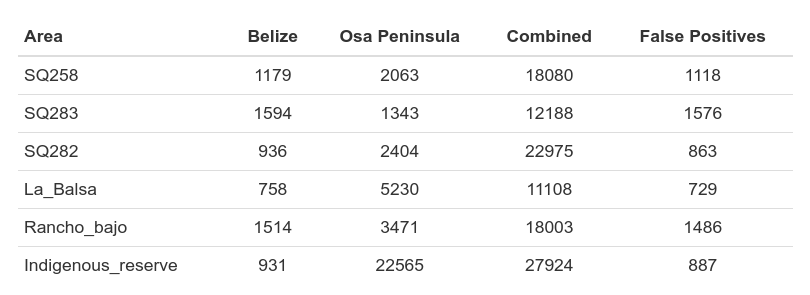
\includegraphics[width=1.2\textwidth,center]{Figures/model_comparison}\caption[Model comparison]{Number of returned 'gunshots' from each version of the convoluted neural network (CNN). The 'Belize' model was trained only on data provided by \cite{Hill2018}, 'Osa Peninsula' was trained on data collected by Jenna Lawson \citep{Lawson2019}, 'Combined' was trained on a combination of the previous two datasets, and 'False Positives' was trained on Jenna's data but all negatives provided were previously identified false positives.}\label{fig:model_comparison}
\end{figure}

\begin{figure}
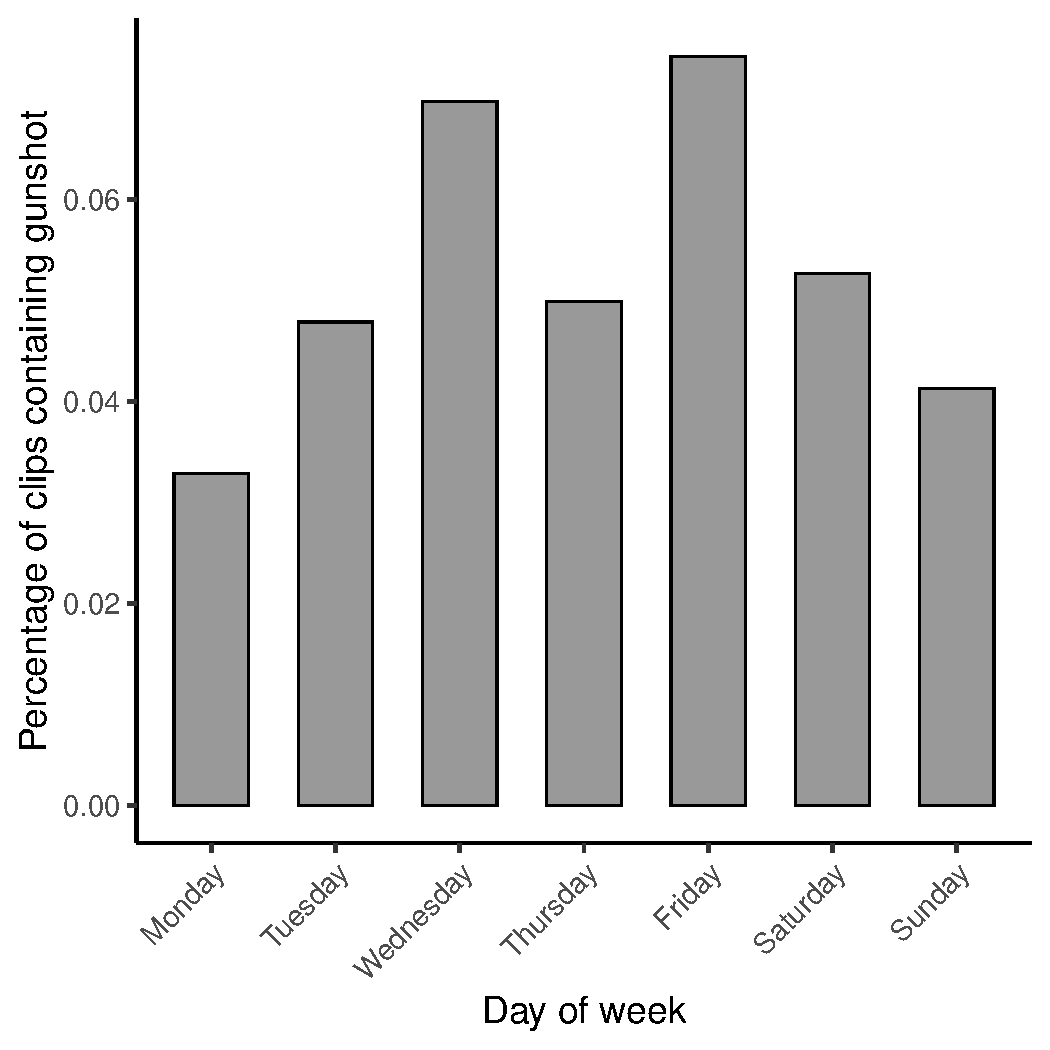
\includegraphics[width=1.2\textwidth,center]{Figures/weekday_plot}\caption[Gunshot frequency by day of week barplot]{Percentage of clips containing a gunshot on each day of the week.}\label{fig:weekday_plot}
\end{figure}

\begin{figure}
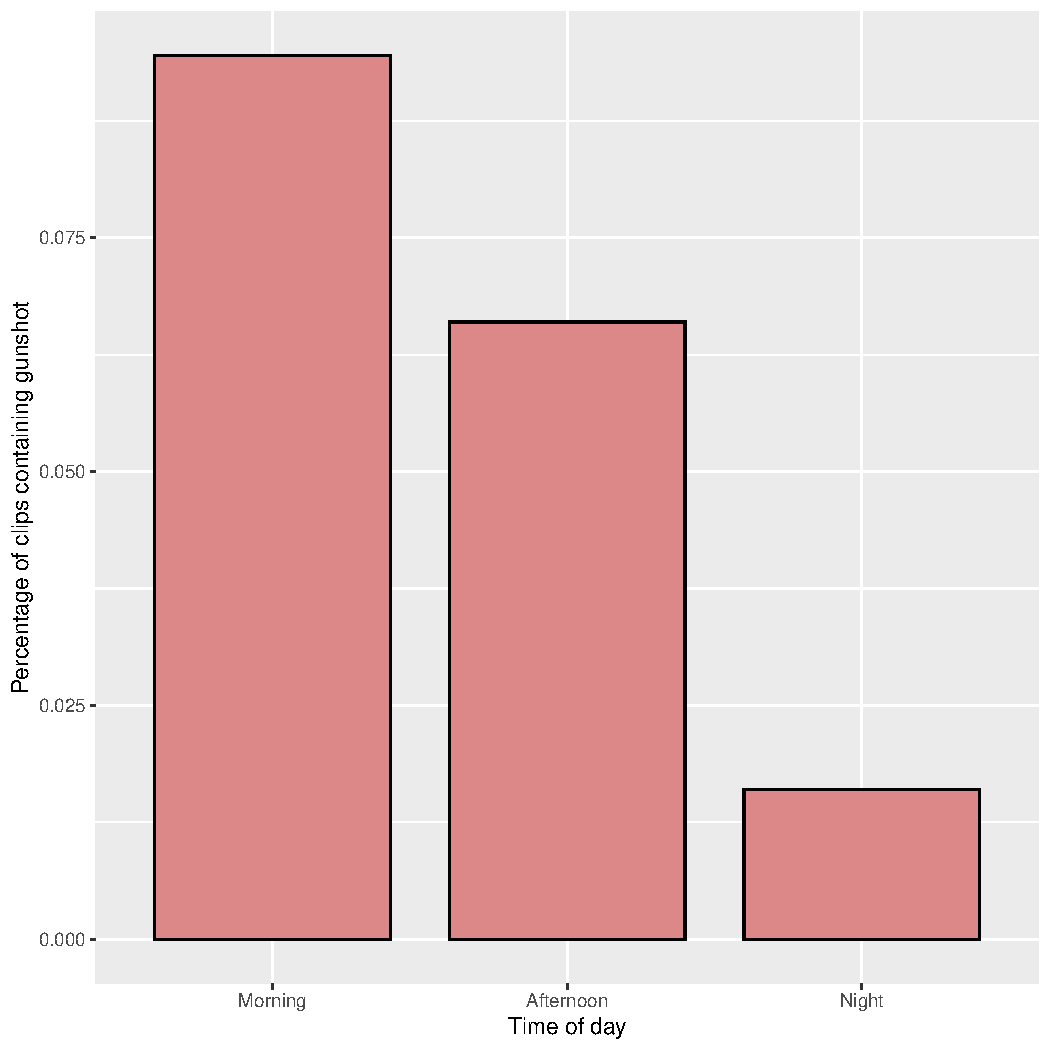
\includegraphics[width=1.2\textwidth,center]{Figures/timeday_plot}\caption[Gunshot frequency by time of day]{Percentage of clips containing a gunshot in each period of the day. 'Morning' was 0500-0930, 'Afternoon' was 1400-1830, and 'Night' was 2100-0300.}\label{fig:timeday_plot}
\end{figure}


\begin{figure}
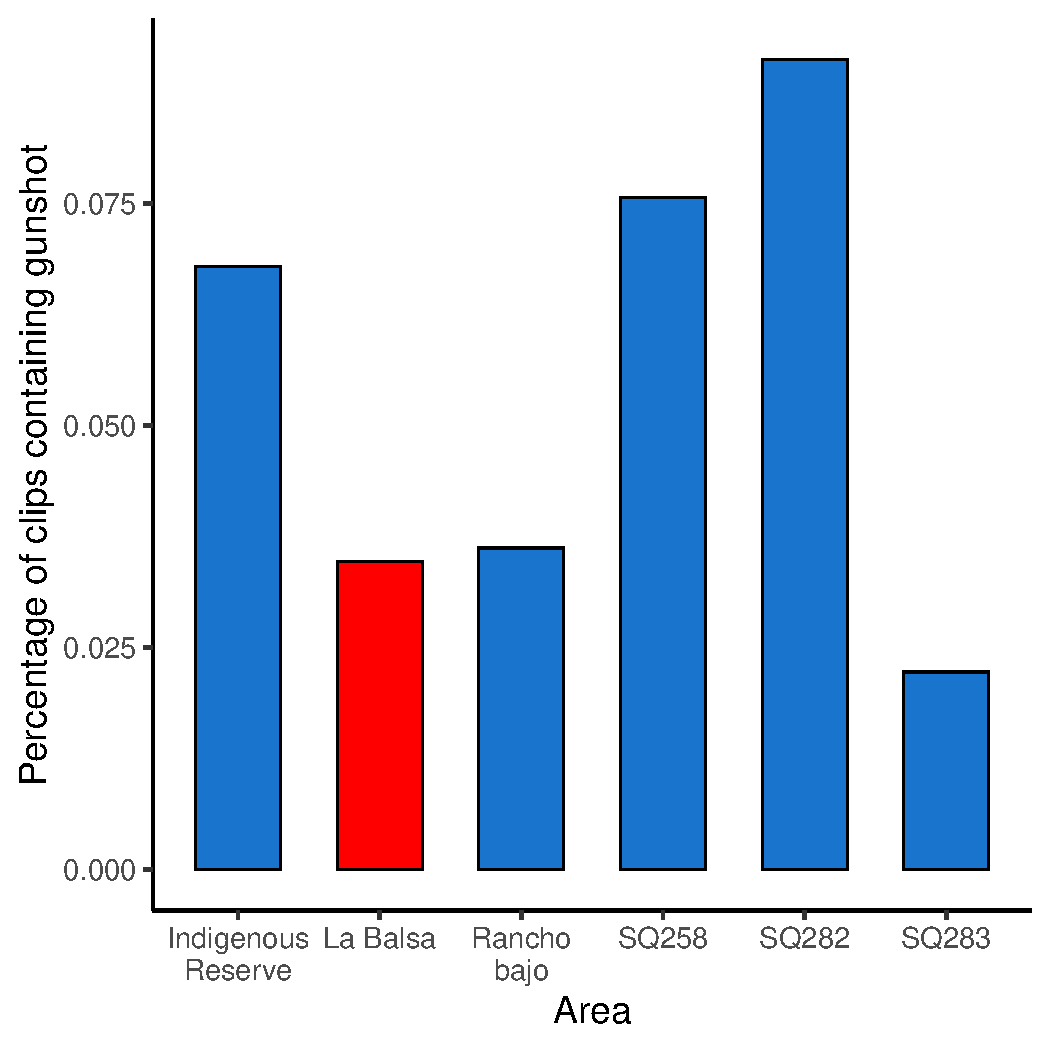
\includegraphics[width=1.2\textwidth,center]{Figures/area_plot}\caption[Gunshot frequency by area]{Percentage of clips containing a gunshot within each of the six regions within the study site.}\label{fig:area_plot}
\end{figure}

% Chapter Template

\chapter{Discussion} % Main chapter title

\label{Discussion} % Change X to a consecutive number; for referencing this chapter elsewhere, use \ref{ChapterX}

\subsection{Machine learning and its effectiveness}
Perhaps surprisingly, training the CNN on the data provided by \cite{Hill2018} was quite effective despite this data coming from a different country at a different time. This success was marred by low precision despite the potentially high recall. However it cannot be said for certain if the recall was high as that would require manual validation of the whole dataset to indentify all the gunshots and thus whether they were successfully identified by the CNN or not. That being said, due to the surprisingly high volume of gunshots identified, it seems logical to assume that the recall was high. Re-training the CNN on both the output of the Belize model and a combination of the Belize and Osa Peninsula data proved ineffective in reducing the volume of false positives returned. However, re-training the CNN on the Osa Peninsual data with the negatives provided being previously identified false positives, seemed to bring the precision in line with, or slightly better than, the Belize model. This strongly suggests that the primary factor in determining the effectiveness of a CNN model in studies such as this is the quality of the dataset used to train the model on. If time had permitted, the logical next step of this study would have been to increase the size of the dataset and continue to retrain the model on an ever larger, more accurate dataset. This may be the only way to improve the precision going forward.


\subsection{Spatio-temporal hunting patterns on the Osa Peninsula}
Correlation between gunshot frequency and the day of the week proved to be insignificant but visual inspection of the data does seem to suggest a non-unfiform distribution across the days and a relatively low p-value suggests this may prove significant if more data was gathered. Similarly, there was no significant correlation between time of day and gunshot frequency but again, chi-squared test results returned a low p-value so the size of the dataset is probably playing a part again. The gunshot frequency was around four times lower at night which seems to suggest non-uniformity and contrasts completely with the findings of \cite{Astaras2017}. This may be due to infrequent patrolling in these areas. Jenna Lawson says that patrols in the national parks are at best once per day in the mornings and usually only cover a small percentage of the total park area so perhaps this is a negligable hinderance to illegal hunters. 


\subsection{Conclusion}

%\include{Chapters/Chapter5}

%----------------------------------------------------------------------------------------
%	THESIS CONTENT - APPENDICES
%----------------------------------------------------------------------------------------

\appendix % Cue to tell LaTeX that the following "chapters" are Appendices

% Include the appendices of the thesis as separate files from the Appendices folder
% Uncomment the lines as you write the Appendices

%% Appendix A

\chapter{Frequently Asked Questions} % Main appendix title

\label{AppendixA} % For referencing this appendix elsewhere, use \ref{AppendixA}

\section{How do I change the colors of links?}

The color of links can be changed to your liking using:

{\small\verb!\hypersetup{urlcolor=red}!}, or

{\small\verb!\hypersetup{citecolor=green}!}, or

{\small\verb!\hypersetup{allcolor=blue}!}.

\noindent If you want to completely hide the links, you can use:

{\small\verb!\hypersetup{allcolors=.}!}, or even better: 

{\small\verb!\hypersetup{hidelinks}!}.

\noindent If you want to have obvious links in the PDF but not the printed text, use:

{\small\verb!\hypersetup{colorlinks=false}!}.

%\include{Appendices/AppendixB}
%\include{Appendices/AppendixC}

%----------------------------------------------------------------------------------------
%	BIBLIOGRAPHY
%----------------------------------------------------------------------------------------

\printbibliography[heading=bibintoc]

%----------------------------------------------------------------------------------------

\end{document}
